% Use this file as a source of example code for your aapm document.
\documentclass[%
 aapm,
 mph,%
 amsmath,amssymb,
%preprint,%
 reprint,%
%author-year,%
%author-numerical,%
]{revtex4-2}

\usepackage{graphicx}% Include figure files
\usepackage{dcolumn}% Align table columns on decimal point
\usepackage{bm}% bold math
\usepackage{multirow}
\usepackage{subcaption}

%\usepackage[mathlines]{lineno}% Enable numbering of text and display math
%\modulolinenumbers[5]% Line numbers with a gap of 5 lines
%\linenumbers\relax % Commence numbering lines

\begin{document}

\preprint{AAPM/123-QED}

\title[DLA Computational Simulation]{Computational simulation of diffusion limited aggregation}% Force line breaks with \\
%\thanks{Footnote to title of article.}

\author{23532}
 %\altaffiliation[Also at ]{Physics Department, XYZ University.}%Lines break automatically or can be forced with \\
%\author{B. Author}%
 %\email{ew639@bath.ac.uk}
\affiliation{ 
Department of Physics, University of Bath, Bath, BA2 7AY, United Kingdom
}%

\date{\today}% It is always \today, today,
             %  but any date may be explicitly specified

\begin{abstract}
Measurements will be made on two different diffusion limited aggregation (DLA) simulations. Using the radial size of the systems they are shown to both produce clusters with the same fractal dimension. Box counting is then used to determine a fractal dimension of $1.716\pm0.007$, a value consistent with numerous published values. The simulation is then modified so that not all particles will aggregate onto the cluster after their first collision. Another modification enables simultaneous simulation of walker particles. Both these modifications caused the fractal dimension to tend towards 2. However an equation was found which, in the latter case of simultaneous particles, described the limit for diffusion to dominate the growth of the cluster.
%
\end{abstract}
%\keywords{Suggested keywords}%Use showkeys class option if keyword
                              %display desired
\maketitle

\begin{quotation}
This report is for PH30056 Computational Physics B: Coursework 1.

Code, figures, data and additional appendices can be accessed at \url{https://edwardwebster.me/?p=370}
\end{quotation}

\section{\label{sec:introduction}Introduction}
Diffusion limited aggregation (DLA) is a process where particles (walkers) diffuse through space which stick together when they come into contact \cite{dictionary} forming a cluster. The cluster formed by a DLA process is commonly seen in natural growth systems\cite{MeakinDLA} warranting studies into the process. DLA was first simulated by Witten and Sander\cite{WittenDLA} and who created a computational simulation of DLA. Since then major advances in computing technology have allowed for much larger simulations to be created.

In their paper Witten and Sander outlined a method for simulating DLA as follows\cite{WittenDLA}. Simulations create individual walkers which undergo Brownian motion. A cluster is initially created with one seed particle. When the walker encounters a clustered particle it joins the cluster and can no longer move. A new walker is generated and this too undergoes random motion until it encounters the cluster. As more particles are simulated like this the cluster grows and measurements can be made on the system. One measure of the produced cluster is its fractal dimension.
\subsection{\label{sec:fractals}Fractals}
Fractals are objects for which the topological dimension\footnote{dimension of space the fractal exists in} is not equal to their fractal dimension\cite{FractalsBook}. Fractals have a non-integer dimension and exhibit a property called self similarity whereby smaller segment of the fractal closely resembles its larger structure.

Conventionally, we are experienced with objects who's dimension ($d$) is an integer (e.g a 1D line or a 2D square) where the object scales with $2^d$. 
%In these cases the dimension is easily assessed by considering how each object scales.
An example is, doubling the length of the sides of a square increases its area by 4 which is $2^2$, thus, the dimension of a square is 2. One could easily compare this to doubling the radius of a sphere which causes the volume to increase by eight, hence $d=3$; or similarly to a line which doubles in length, $d=2$. 

Unlike these objects, the calculated dimension of a fractal is not an integer. There are numerous methods which can be employed to determine a fractals dimension. One method of calculating the dimension of a fractal is box counting, where the fractal is observed on successively smaller grid's of boxes and the number of boxes containing a fragment of the fractal counted (see appendix \ref{ap:box_counting}). Alternatively, another method counts the number of points, $N$, of size $a$ required to construct an object which has a radius of $R$. The fractal dimension in this case is
\begin{equation}
\label{eq:FractalDimensionRelation}
N = \left ( \frac{R}{a} \right )^d,
\end{equation}
where $d$ is the fractal dimension\cite{CompBCoursework}. 
%The equivalence of these two techniques to establish the fractal dimension will first be verified. Assuming the two methods yield the same result, box counting will be used as the main technique to measure the fractal dimension.

%An analysis will also be made for systems which start with multiple seed particles.
\section{\label{sec:simulation}DLA Simulation}
A simulation was ran in C++ which simulated the DLA system described in section \ref{sec:introduction}. Code was provided by A.Souslov and V.Rimpilainen which simulated the system\cite{CompBCoursework}. Small modifications were made to their code with these modifications and full code available on GitHub
%REFERENCE
.

A second new simulation was created with a few key differences to previous method. These differences will be explained in section \ref{sec:new_code}. The values for the sticking probability and kill radius remained at the values used by A.Souslov and V.Rimpilainen for comparison with a new approach developed to simulate the process.
\subsection{\label{sec:previous_code}Previous Method}
The simulation provided by A.Souslov and V.Rimpilainen creates a seed particle at the origin of a grid. Particles are then created one at a time which undergo random step in the $x$ or $y$ direction at each time step. When the particle encounters a clustered particle it ceases to move and joins the cluster, at which point a new particle is created. As described in Witten and Sander's paper\cite{WittenDLA} the simulation runs quicker\cite{CompBCoursework} by generating particles on a circle at a fixed distance from a circle who's radius is equal to the furthers cluster particle from the origin. Likewise, the simulation is also sped up by resetting any particles who exceed another circle at a further distance ($r_{kill}$) from the origin (see figure \ref{fig:witten_dla_system} in appendix \ref{ap:witten_dla})\cite{CompBCoursework}.

%New particles are created at a constant distance from the maximum size of the cluster. Any particle which exceeds a specified distance from the cluster radius is destroyed - as it will take a long time to get back to the cluster - and a new one generated to take its place. These methods are designed to speed the simulation up.

Finally, the fractal dimension is calculated from the number of particles forming the cluster. The radius of the furthest clustered particle ($r_{max}$) from the origin is used to calculate fractal dimension from the number of particles in the cluster ($N$). From equation \ref{eq:FractalDimensionRelation} the fractal dimension is found from the gradient of the line of best fit connecting $\ln(N)$ against $\ln(r_{max})$. According to equation \ref{eq:FractalDimensionRelation}, these should be related by
\begin{equation}
\ln(N)=d \ln(R) + \ln(\beta),
\end{equation} 
hence, the gradient should measure the fractal dimension. The simulation was ran numerous times, each time creating a different fractal, and the dimension finally determined from the average of these runs.

Modifications were made to the code which allowed the sticking probability to take effect. Instead of every `collision' with the cluster aggregating, a certain probability was defined in order for particles to stick. Particle's which did not stick kept on walking. Simulations revealed that the sticking probability and kill radius influenced the fractal dimension.
\subsection{\label{sec:new_code}New Method}
A new simulation was created to simulate the system. A two dimensional grid of zeros was created which represented positions of the particles in the cluster. A seed was initiated at the origin. Walkers were generated which randomly walked until they encountered the seed (or cluster) at which point they aggregated onto the system turning the position in the grid to a one instead of a zero.

The new simulation differed from the previous method as the size of the grid could be easily changed. The boundaries of this grid could also be modified so that particles bounced off of the boundary, or the made periodic so that particles which tried to leave the right hand side of the system reappeared on the left. In the previous method the boundary was never a concern since the kill circle prevented this distance from being reached. Unless stated the periodic boundary was used, although, no difference was measured in the fractal dimension under both conditions. In addition, the new simulation allowed for more control over the position of the seed and number of seed particles (see fig). For the simulations explored in this paper only one central seed particle is used. As in the previous method, the sticking probability was also able to be modified.

Under the conditions stated, one would expect the two simulations to produce the same fractal since neither differ in the growth mechanism nor properties of the system. The final change to the simulation was the simulation of the walker particles. Under the new method, walkers\footnote{walkers could also travel a cell diagonally which wasn't possible in the previous method} could either be generated individually until they contact the cluster (as already explored in section \ref{sec:previous_code} by A.Souslov) or all the particles could be generated and diffuse simultaneously. As such a new property was introduced into the system, the area density of walker particles, $\rho$. The grid was filled with particles at a density $\rho$ in random positions. On contact with the cluster, the particle would stick and then a new particle would be created at a random position. If the new position was on or contacting the cluster, the particle was abandoned. By creating new walkers when the particle joins the cluster, and discarding particles inside the cluster the density was kept constant throughout the simulation to within 2\% of the specified density.
%
% In order to conduct further analysis a new code was created. A grid who's size could be specified was initialised with seed particles also specified (normally the origin was used). Random particles were created and at each time step allowed to take independent steps in $x$ and $y$ (allowing for diagonal steps which previously could not be taken). When a particle collides with the cluster it became inactive and joined the cluster. Notably the following properties of the system could be controlled:
% \begin{itemize}
%     \item the geometry of the simulation
%     \item the seed position's and number of seeds
%     \item the probability of walker sticking to the cluster/seed
%     \item the interactions of walkers
%     \item number (density) of walker particles
% \end{itemize}
% which were not previously accessible using the method from A. Souslov.
%
% The process by which the cluster formed by DLA grows will be investigated in many scenarios. Initially, the fractal dimension of the `base' case will be measured - this is the dimension of a cluster which grows when a single particle is simulated at a time. The dimension of a cluster which is grown from many non-interacting particles at a given density will be simulated, with the aim of determining how the change in density of particles affects the growth of the cluster. Finally, the same approach will be taken for many particles, however, the growth of the cluster will be analysed as a function of density for many particles which do interact such that they can not occupy the same position.
%
\section{\label{sec:fractal_dimension}Measuring the Fractal Dimension}
There were two different techniques which could be used to measure the fractal dimension of the cluster. The first, referred to as radial fractal dimension, is implemented by applying equation \ref{eq:FractalDimensionRelation} to the cluster, using the distance of the furthest point from the origin as the measure of the radius\cite{CompBCoursework,MeakinDLA,FractalsBook}. Calculating the radial fractal dimension is commonly used in DLA\cite{FractalsBook,MeakinDLA,WittenDLA}.

An alternative method is box counting\cite{CompACoursework} which uses the same scaling principle but counts the number of occupied boxes in grids of different scales. Box counting is particularly useful when the radius of the system is not easy to asses.

In the following sections (\ref{sec:radial_fractal_dimension} and \ref{sec:box_counting}) a comparison of the two techniques will be made and assessed for use in the investigation.
\subsection{\label{sec:radial_fractal_dimension}Radial Fractal Dimension}
Using the provided code by A.Souslov and V.Rimpilanen a DLA cluster is grown to 3500 particles. The maximum radius ($r_{max}$) and number ($N$) of cluster particles is written to a \verb+.csv+ as the program runs. A linear fit of the logarithm of these values according to equation \ref{eq:FractalDimensionRelation} is applied. Based on the described measure of the fractal dimension, the previous method is found to have a fractal dimension of $1.7553 \pm 0.0231$.

Using the same technique, the fractal dimension of a cluster using the new simulation code where particles are singularly generated had a fractal dimension of $1.7568 \pm 0.0159$.

\begin{figure}[h]
\centering
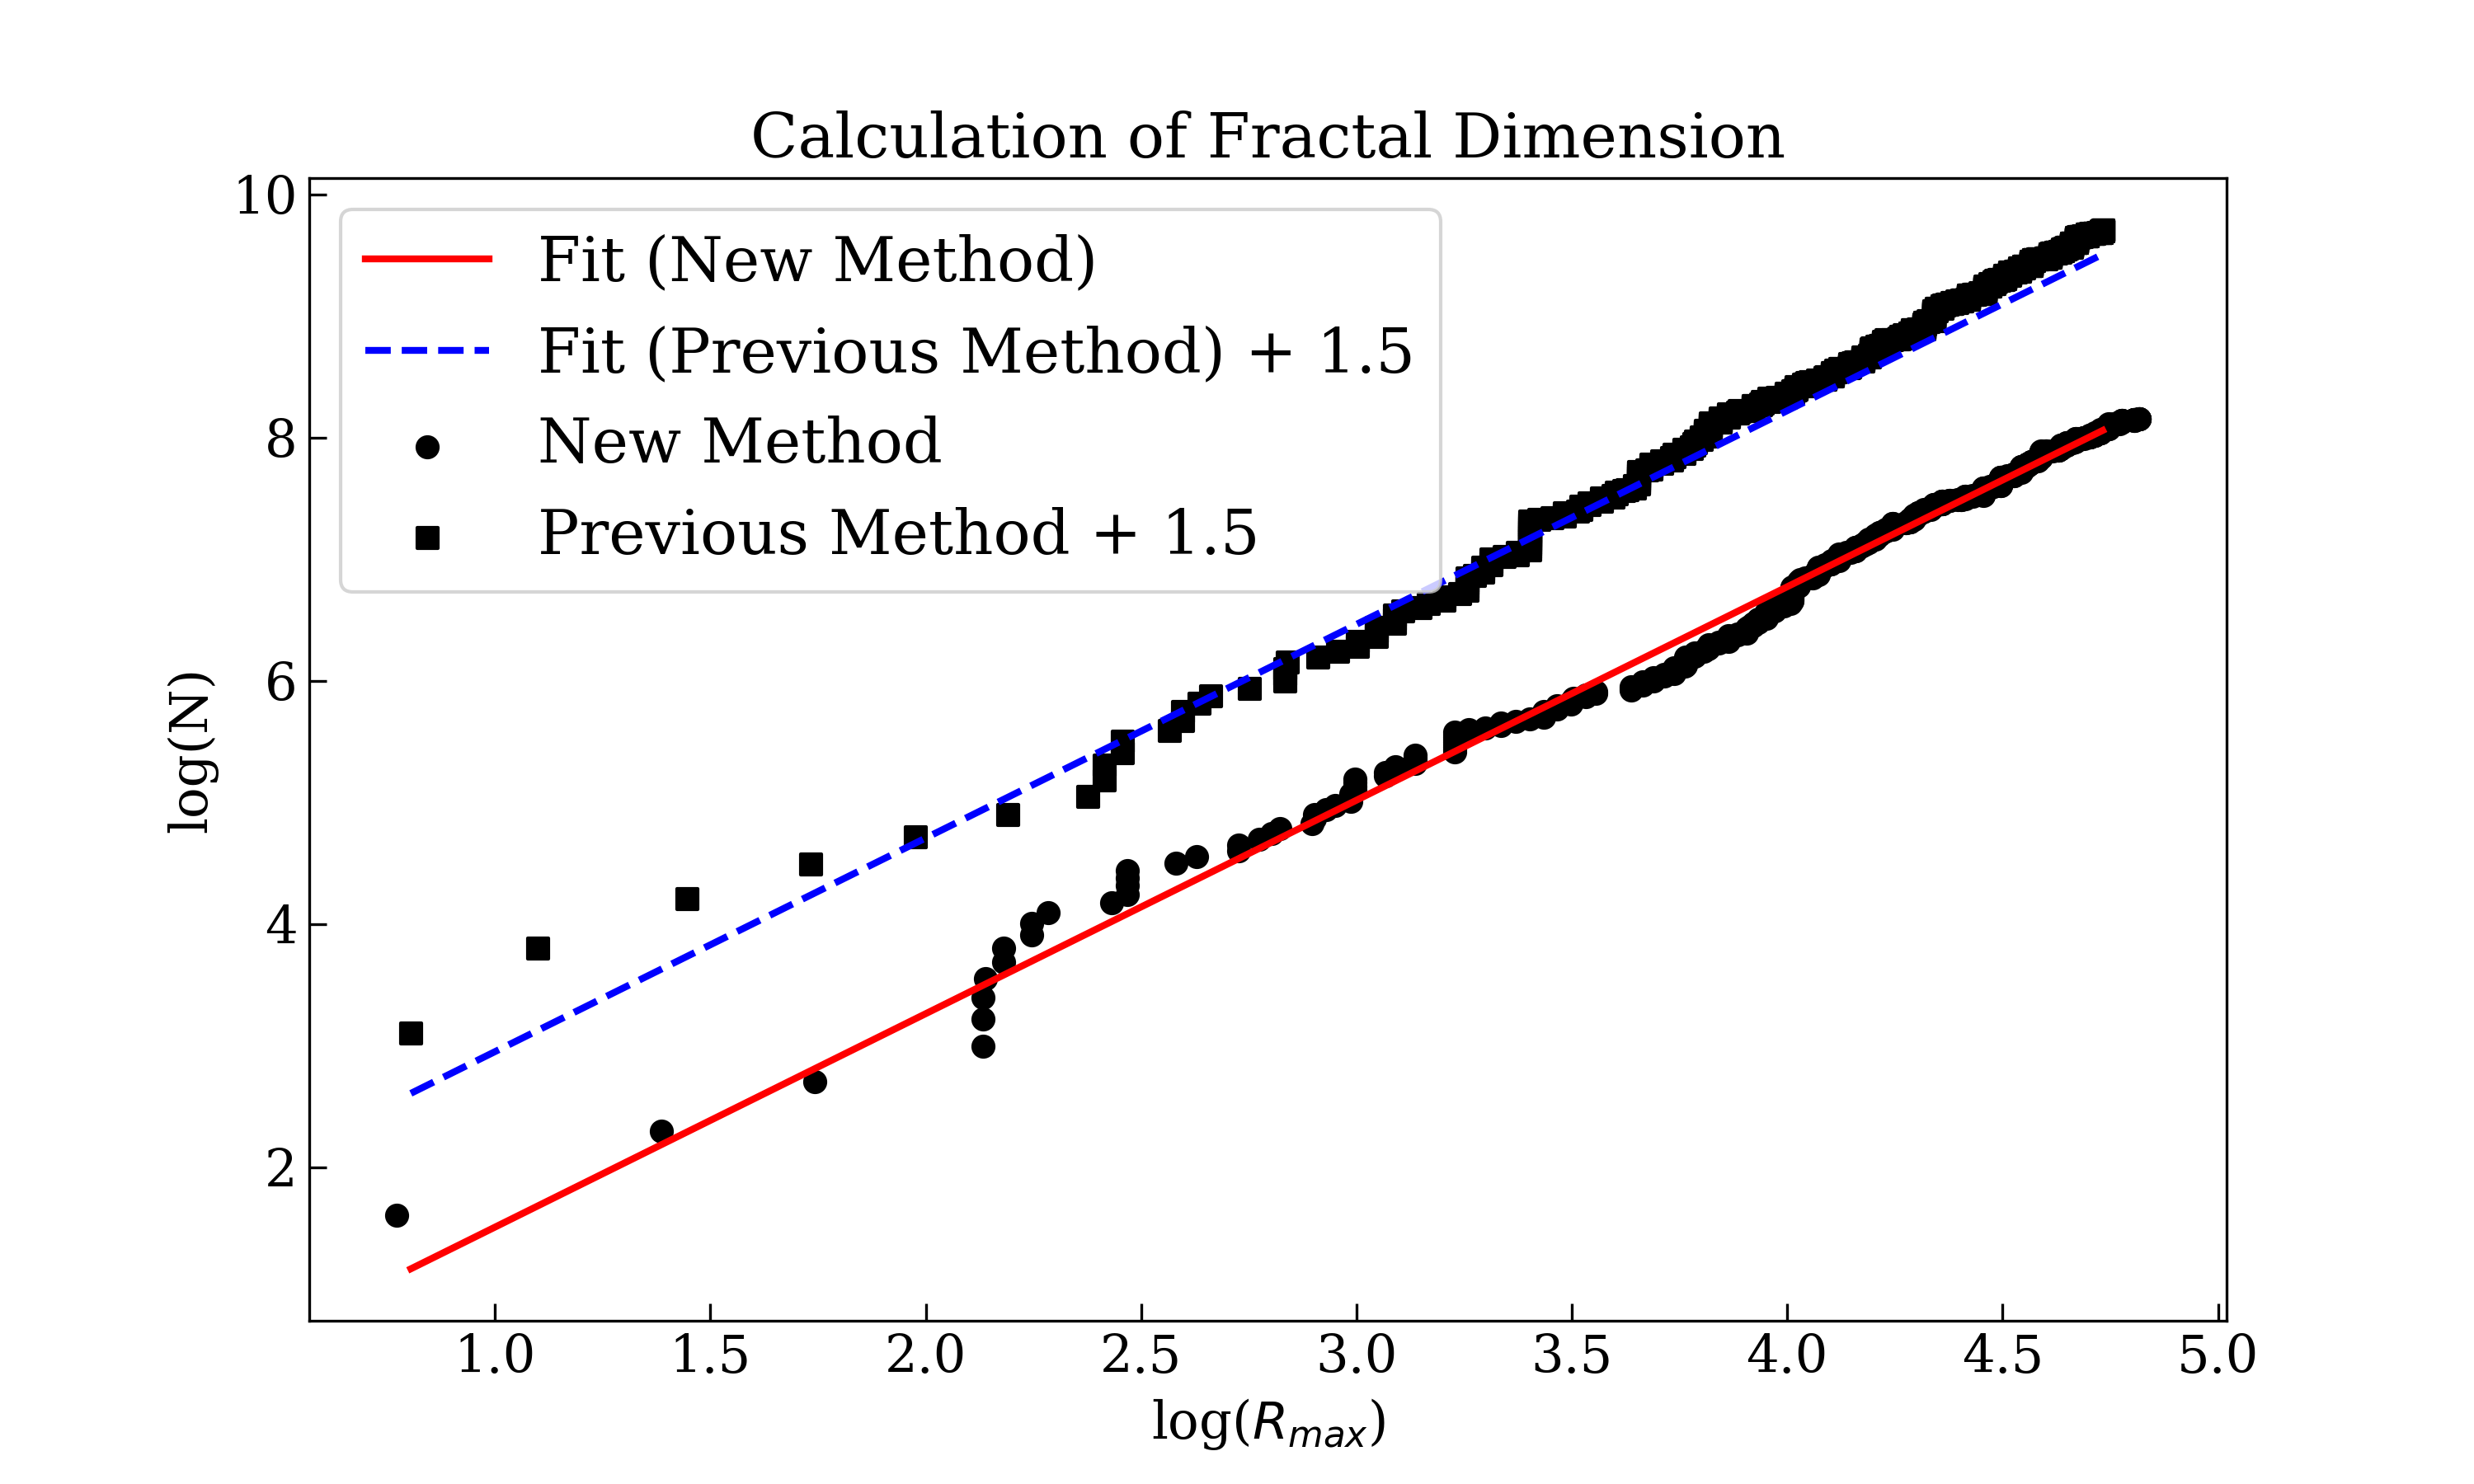
\includegraphics[width=\linewidth]{figures/1.png}
\caption{\label{fig:radial_dimension}Plot used to perform a linear fit to the radial data. The values for the original method has been offset by 1.5 units to increase the clarity of the diagram. The fractal dimension of the cluster is obtained from the gradient.}
\end{figure}
These measurements are a promising indication that the new simulation properly implements the DLA method. Within the measurement uncertainties both simulations produce the same fractal dimension for singularly generated particles.

The uncertainties in the measurements above were obtained from the co-variance matrix of the linear fit which was performed using the \verb+polyfit+ function provided with the widespread \verb+numpy+ package in python. Repeats of the code yielded fractal dimensions which varied in values significantly less than the uncertainties in the linear fit. As such the uncertainty above is an average of the linear fit variances for 10 code reruns.

Having shown that the different simulations have the same fractal dimension under this method, the fractal dimension using box counting was then measured.
\subsection{\label{sec:box_counting}Box Counting Fractal Dimension}
Another method of calculating the fractal dimension of an object is box counting \cite{FractalsBook}. Box counting, as the name implies, counts the number of occupied boxes when the fractal is placed on a grid. The size of grid boxes is then reduced and the number of occupied boxes once again counted. The number of occupied boxes scales with,
\begin{equation}
d = \lim_{\epsilon->0} \frac{ \log N(\epsilon) }{ \log 1/\epsilon }
\end{equation}
where $d$ is the fractal dimension, $N$ the number of occupied boxes as a function of the scale of the boxes $\epsilon$ \cite{FractalsBook,CompACoursework}. As in the radial method, a linear fit is used for grid of 1 to 30 boxes and the fractal dimension obtained from the gradient.

Unfortunately, due to the output style of the previous method, the fractal dimension could only be calculated using box counting for the new simulation. However, the previously made measurement using the radial method had demonstrated that within the measurement uncertainties the DLA clusters grown in the two simulations should have the same dimension.

Box counting has the advantage of a lower uncertainty than the radial method used to calculate the fractal dimension. Using box counting to assess the fractal dimension, the DLA simulation had a fractal dimension of $1.716 \pm 0.007$. Again, the uncertainty specified here was based on the uncertainty in the linear fit as the repeated results showed a smaller deviation than this measurement. Indeed, the value calculated is consistent with the published 1.71 \cite{FractalsBook,MeakinDLA}.

By using box counting to asses the fractal dimension, the measurement uncertainty was halved as opposed to the the radial method. In addition, there was a systematic error causing the radial dimension to be higher than the widely accepted value. In order to reduce the error in the radial fractal dimension, clusters with a large radius must be explored. However, as the cluster grew the radius grew less rapidly, consequently, the simulation time became larger.

The new method was quicker to run allowing for much larger simulations to be created. As such, larger simulations with lower uncertainties could be created. Importantly, box counting required a sufficient number of particles in the cluster so that on the scale of the box grid, the fractal always appeared continuous. As the box size approached the scale of points on the fractal the count of occupied boxes saturates and the technique breaks down. Before this limit box counting had a lower uncertainty than its radial counterpart.
\section{Investigation}
Two main lines of enquiry were explored for the grown the of the system; how the probability of a particle sticking to the cluster affected the growth of the cluster; and how the density of surrounding particles influenced the growth of the cluster.

Initially, the effect of the sticking probability was determined.
\subsection{Sticking Probability}
The effect of the sticking probability was implemented by generating a random floating point number between 0 and 1. If this number was less than the user defined sticking probability the particle would aggregate onto the cluster, otherwise it would keep on walking. By allowing the particle to keep walking it now had the option to `diffuse' towards the cluster centre. Under this circumstance, one would expect to create a denser cluster with a higher fractal dimension (as the filled cluster now resembles a two dimensional object).

Visually, the shrinkage and cluster filling was observed in both simulations. The improved accuracy of the box counting technique and faster simulation times meant that measurements were conducted using the new method and box counting. However, the growth of the radius is also shown as the effect should be visible using both techniques.
\subsubsection{\label{sec:sticking_results}Results}
As expected, the growth rate of systems with lower probabilities was much slower than when all particles stick ($p=1.0$). This result is understood as the expected number of `collisions' must be far greater in order for a particle to stick.

\begin{figure}[h]
\centering
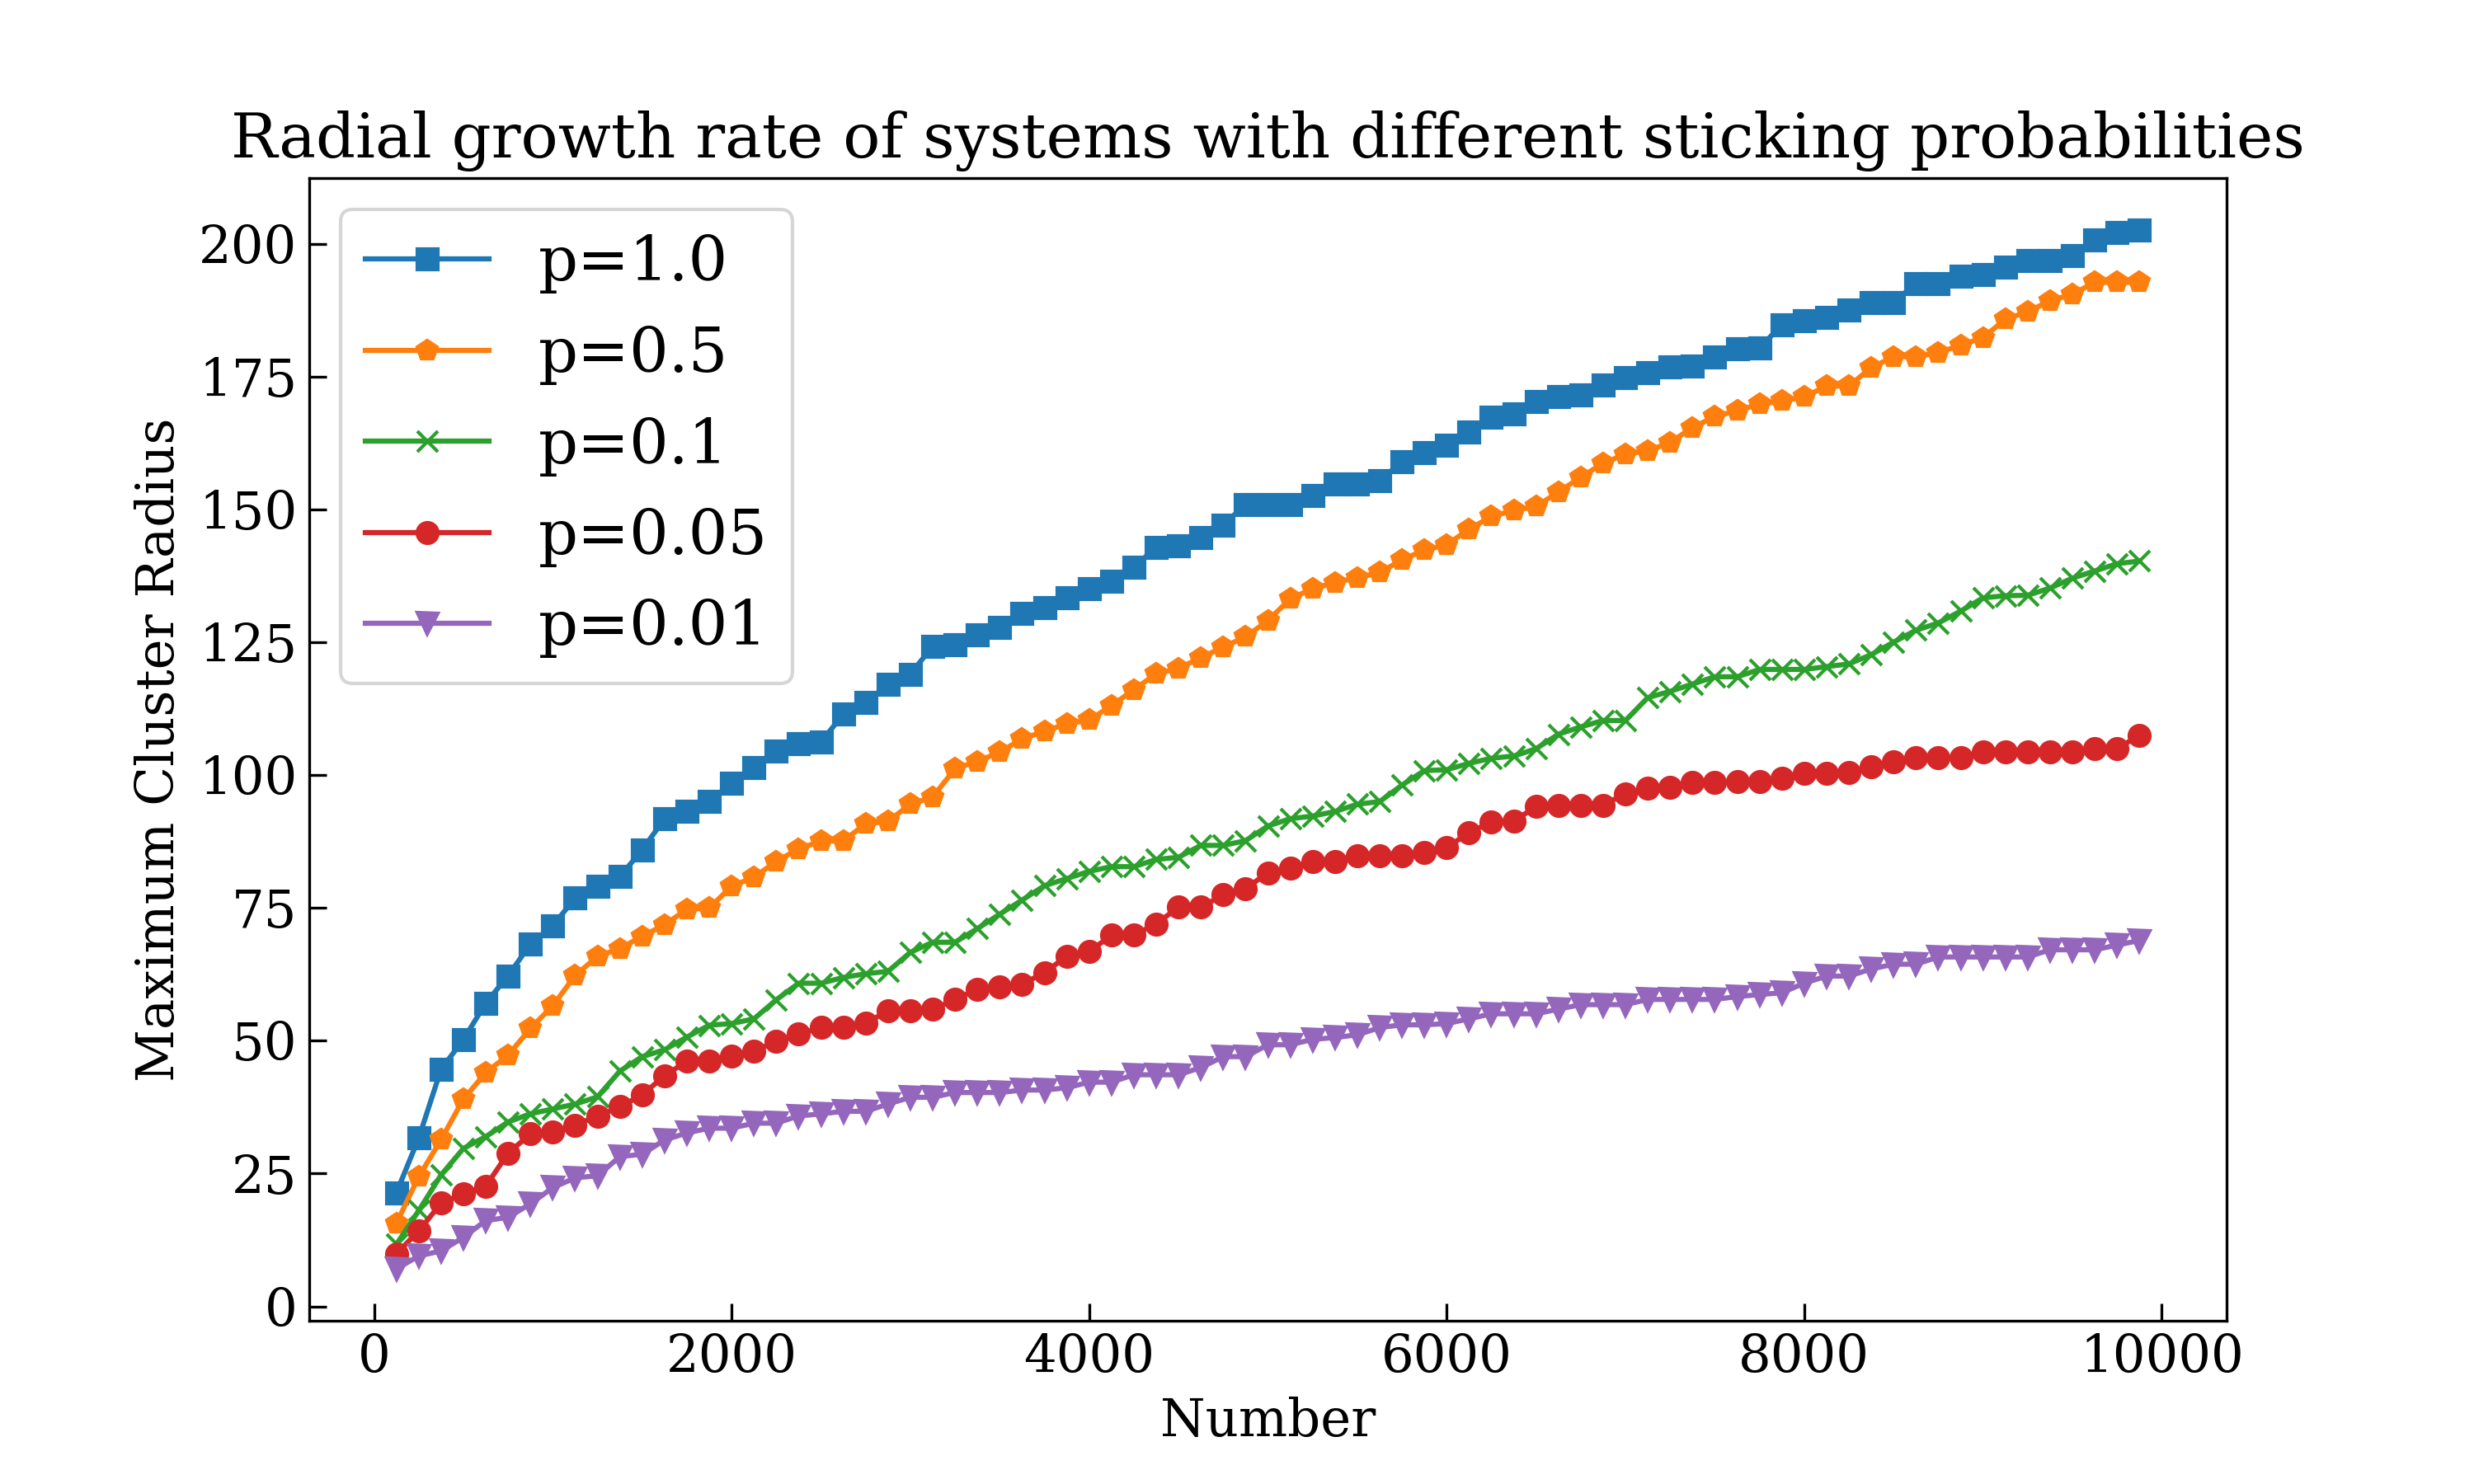
\includegraphics[width=\linewidth]{figures/2.png}
\caption{\label{fig:probability_growth}Clusters with a lower sticking probability were smaller for the same number of particles. Simulations were generated in 14.42, 17.11, 24.97, 28.11 and 40.93 seconds in order of decreasing probabilities.}
\end{figure}
The slowed growth of the system is shown in figure \ref{fig:probability_growth}. Systems with a lower sticking probability were smaller relative to the number of particles contained in the cluster. From figure \ref{fig:probability_growth} it can be seen that a log-log plot would reveal an increasing fractal dimension for systems with a decreased sticking probability.

Using box counting, clusters with sticking probabilities matching those in figure \ref{fig:probability_growth} were grown.
% Please add the following required packages to your document preamble:
% \usepackage{multirow}
\begin{table}[h]
\caption{\label{tab:sticking_probabilities}Decreasing the sticking probability increases the fractal dimension which tends towards a two dimensional object.}
\begin{ruledtabular}
\begin{tabular}{lcr}
\textsc{Sticking Probability}      & \multicolumn{1}{l}{\textsc{Fractal Dimension}} & \multicolumn{1}{l}{($\pm$)} \\ \hline
\multicolumn{1}{c|}{1.0}  & 1.707                                 & 0.011                       \\
\multicolumn{1}{c|}{0.5}  & 1.730                                 & 0.022                       \\
\multicolumn{1}{c|}{0.1}  & 1.806                                 & 0.005                       \\
\multicolumn{1}{c|}{0.05} & 1.865                                 & 0.025                       \\
\multicolumn{1}{c|}{0.01} & 1.941                                 & 0.039                      
\end{tabular}
\end{ruledtabular}
\end{table}
Indeed, these results verified the ansatz made that decreasing the sticking probability increased the fractal dimension. In fact, the fractal dimension tends to a value of 2.0, an unsurprising result since a cluster with no gaps would be a two-dimensional circle. Running the simulation, it was evident that systems with a lower sticking probability did tend towards the two-dimensional case of a filled in circle (this filling in of the cluster is shown in figure \ref{fig:DLAClusters}).
\begin{figure*}[ht]
\begin{subfigure}{0.45\linewidth}
\centering
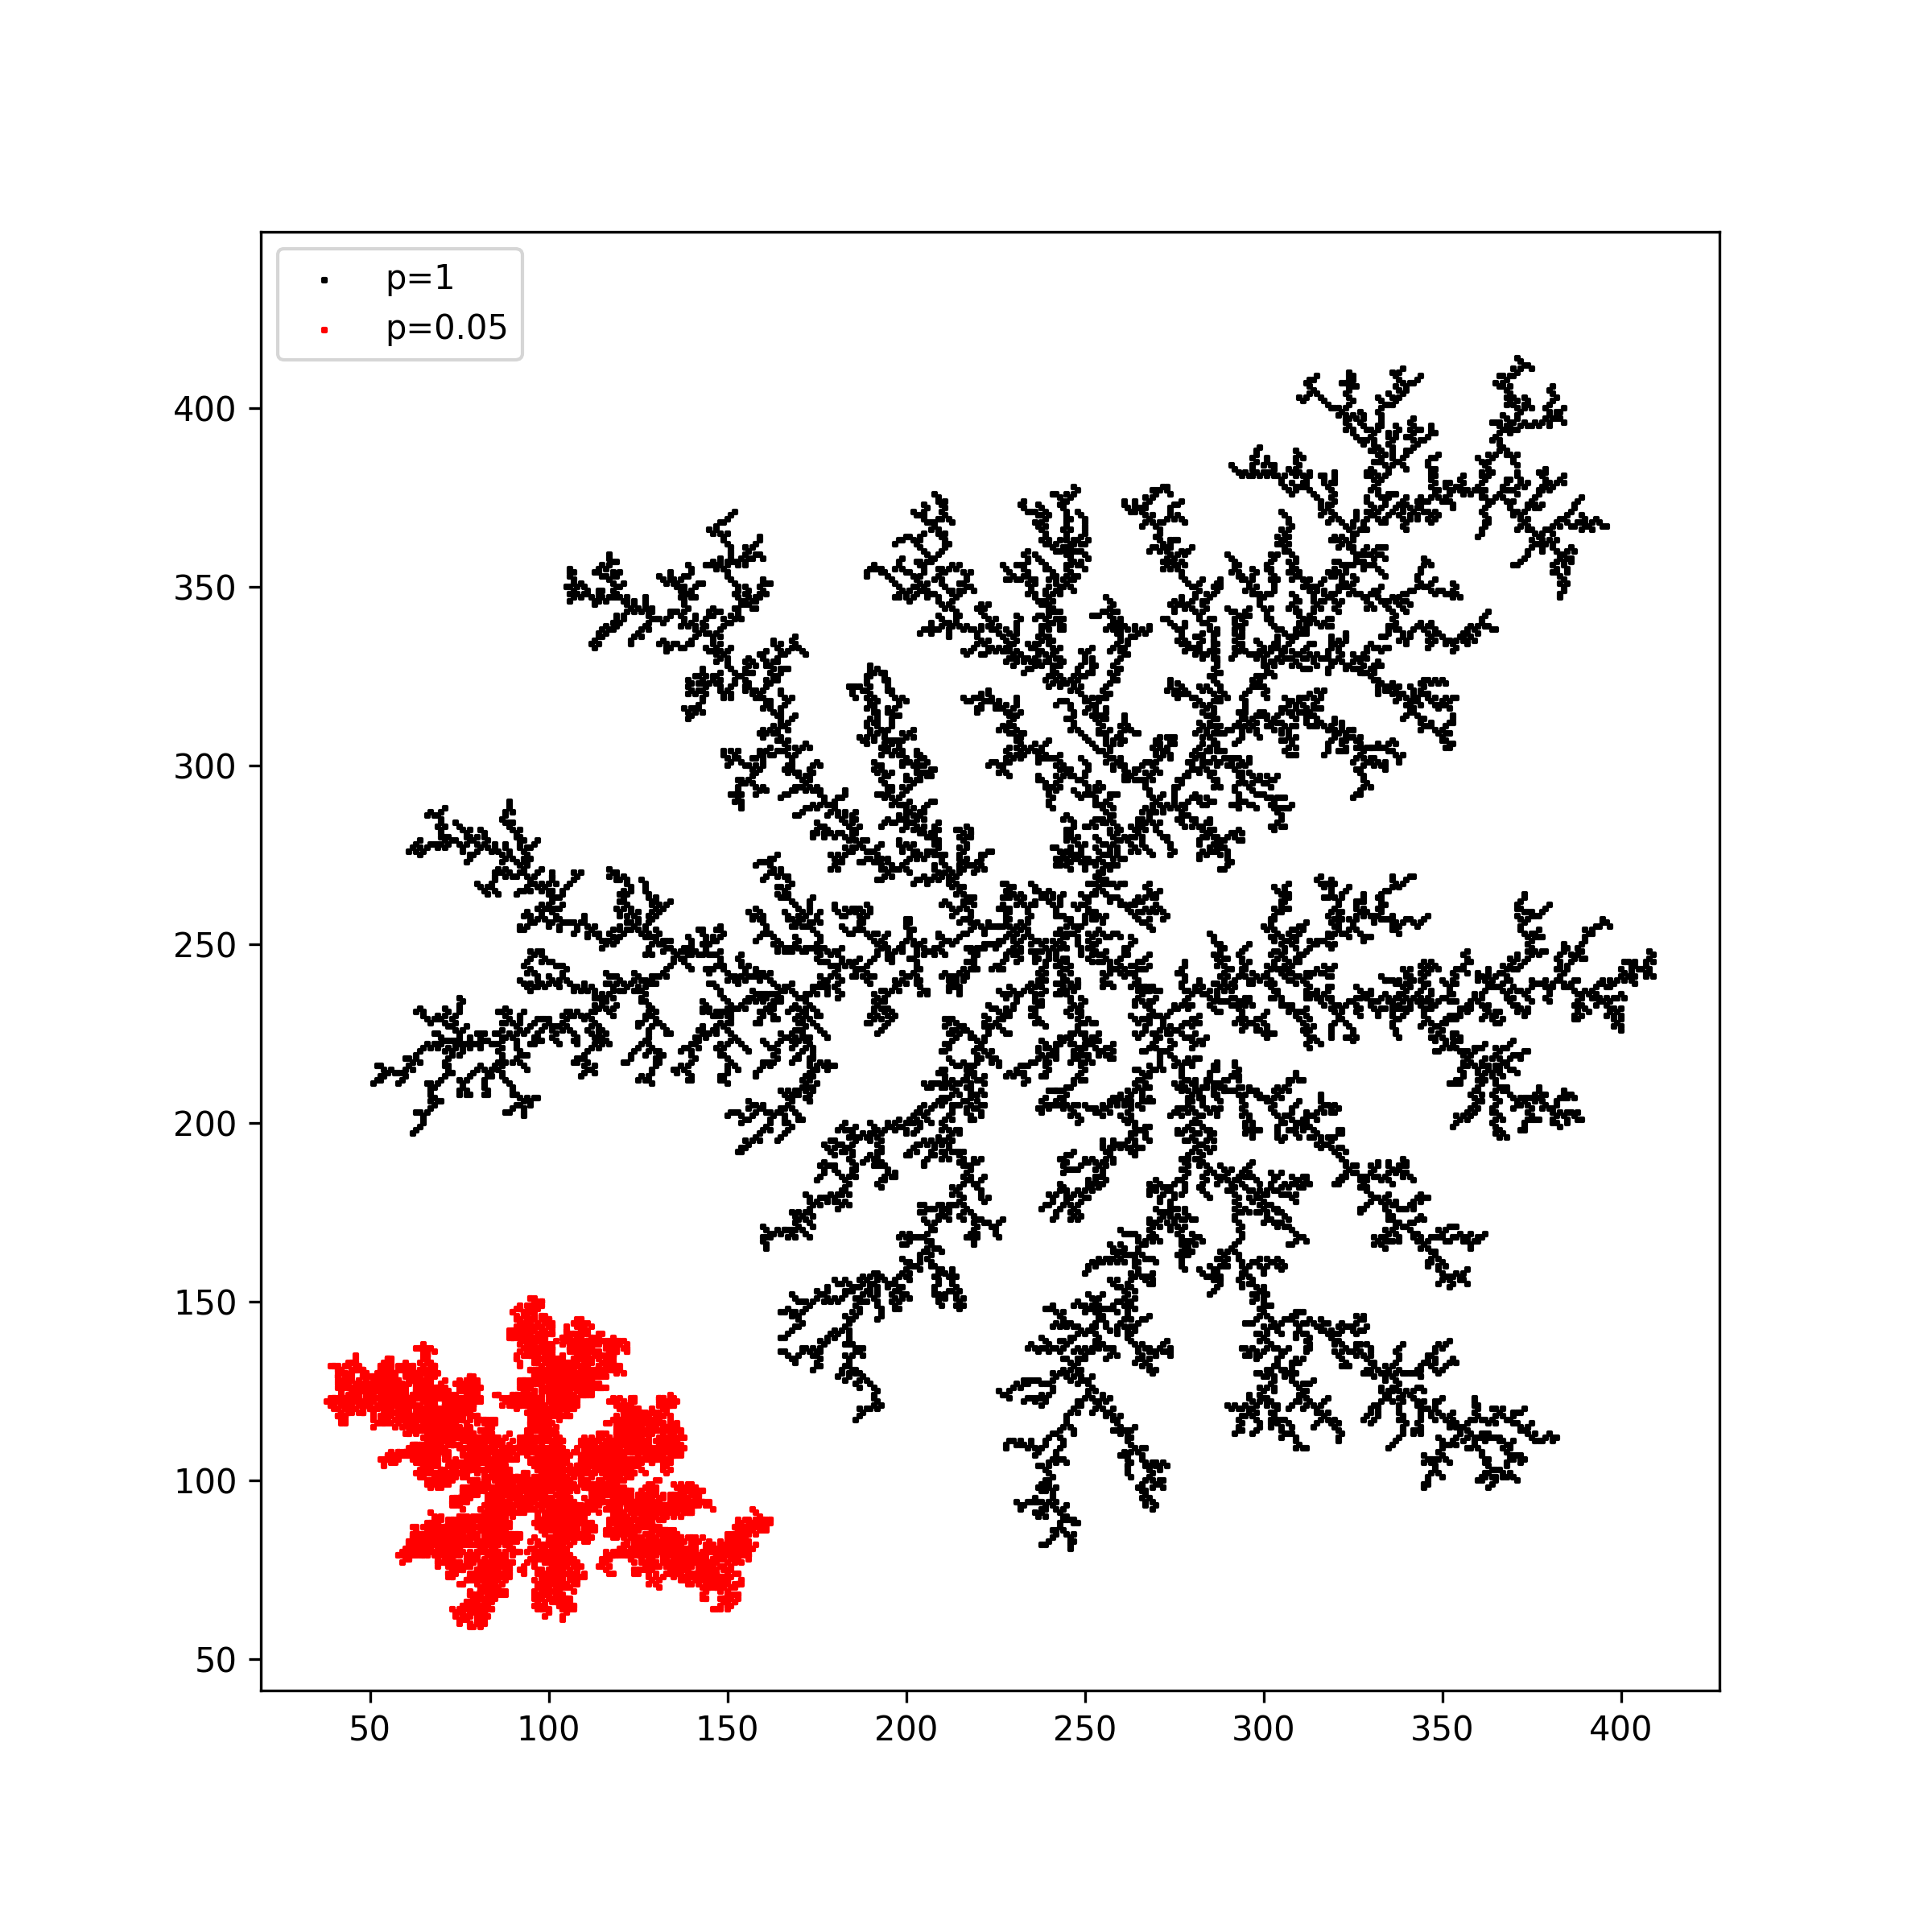
\includegraphics[width=1.0\linewidth]{figures/3.png}
\caption{\label{fig:DLA1,0.05}Simulated DLA clusters for sticking probabilities of 1.0 and 0.05. The later has been offset and coloured red to increase the visibility.}
\end{subfigure}
\begin{subfigure}{0.45\linewidth}
\centering
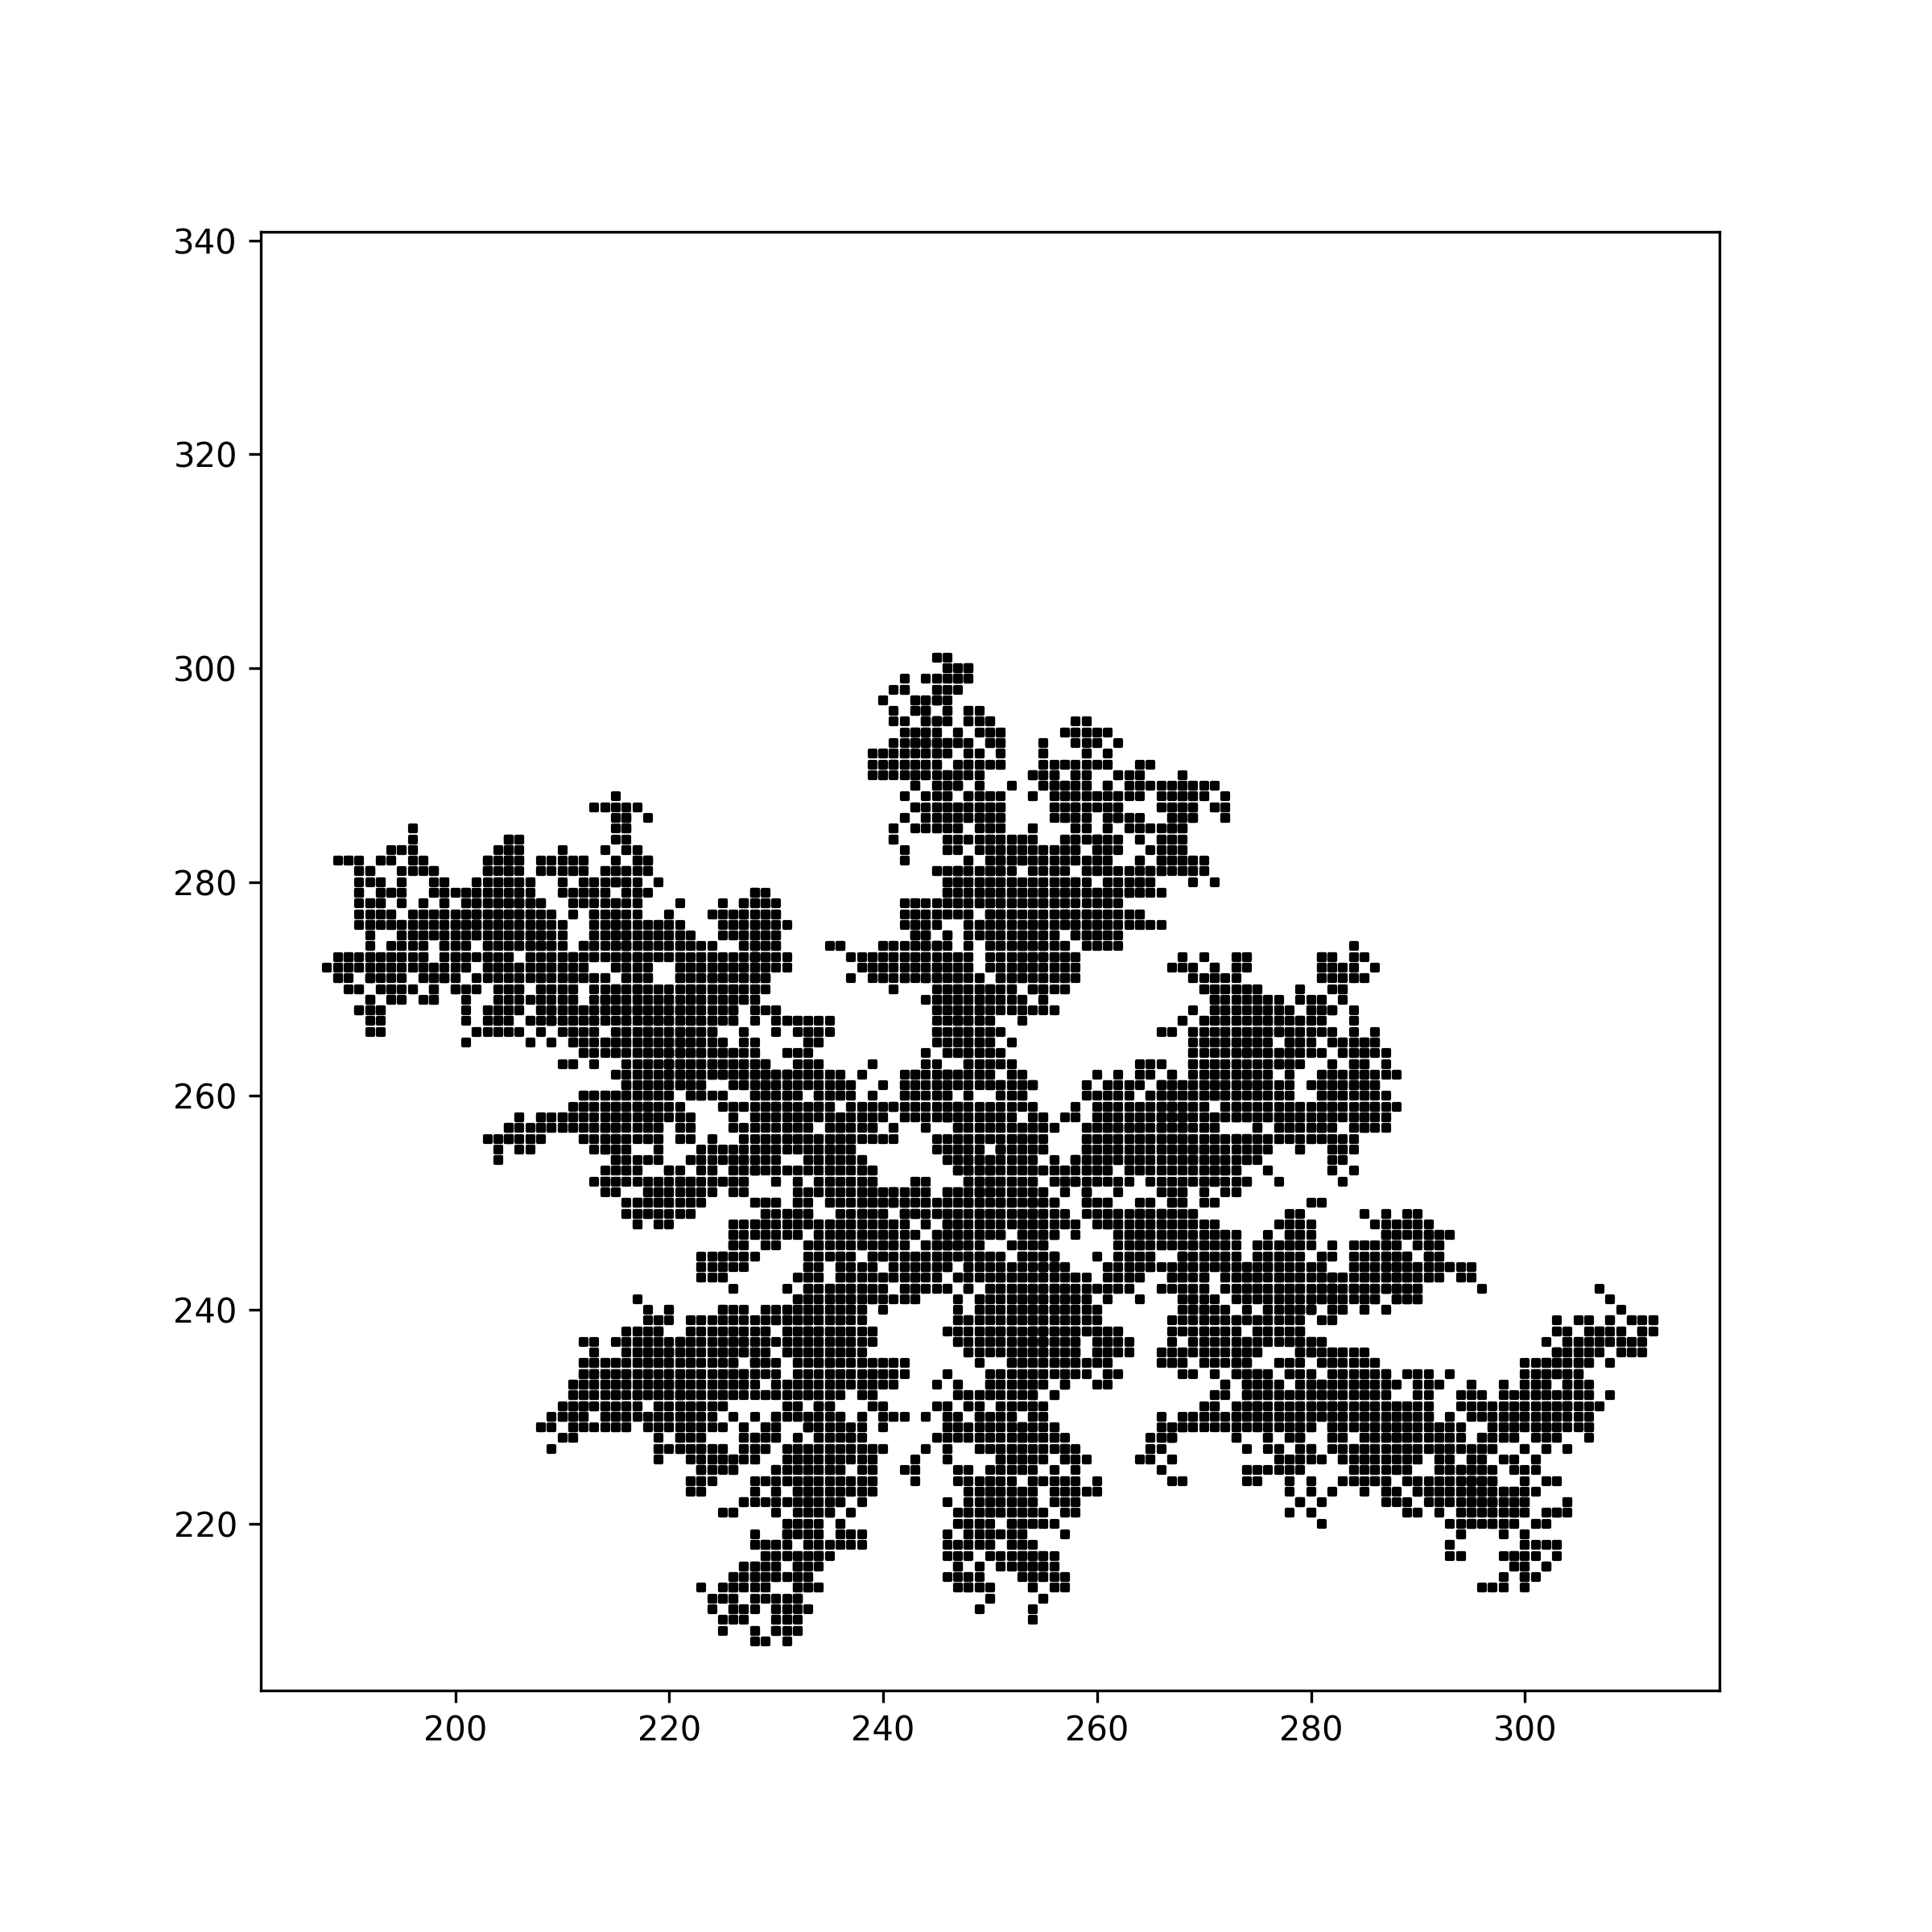
\includegraphics[width=1.0\linewidth]{figures/4.png}
\caption{\label{fig:DLA0.05}Zoomed in image of DLA cluster with a sticking probability of 0.05. The cluster is shown in red figure \ref{fig:DLA1,0.05}.}
\end{subfigure}
\caption{\label{fig:DLAClusters}Simulations of DLA clusters with sticking probabilities of 1.00 and 0.05. The later is much smaller and a scaled up version plotted in figure \ref{fig:DLA0.05}. Compared to the cluster which all particles aggregate the lower sticking probability is smaller and denser with more gaps filled in.}
\end{figure*}
\subsection{\label{sec:density_simulation}Density}
The DLA simulation was then modified slightly. Instead of generating particles individually, a set number of particles were generated at $t=0$ where $t$ is the simulation time. At each time step every particle took a random step as specified in \ref{sec:new_code}.
%If a walker neighboured a clustered particle it was then aggregated onto the system. Periodic boundary conditions were also imposed so a particle walking off of the left of the grid appeared on the right. As such a constant two dimensional density was obtained. 

These walkers did not interact with each other - a condition which was true for the singularly generated particles who had no experience of particles subsequently generated. In the low density limit this condition was assumed to be a good approximation - as the chance of interacting with another walker was low, especially as the cluster grew in size. The density of walkers was given by the equation
\begin{equation}
\label{eq:density}
\rho=\frac{n}{wh},
\end{equation}
where $n$ is the number of walkers, $w$ the width of the grid the walkers are contained in and $h$ the height. Unless stated the width and height of the system were 500 units by 500 units.
\subsubsection{\label{sec:density_results}Results}
DLA clusters were grown as a function of the density of walkers on the grid. In these simulations the sticking probability was kept constant at 1.00 so as not to skew the results by causing all of the fractal dimensions to tend towards 2.0. Table \ref{tab:density_dependence} contains the calculated fractal dimension for walker particles at different densities over 10,000 time steps.
\begin{table}[h]
\caption{\label{tab:density_dependence}Decreasing the sticking probability increases the fractal dimension which tends towards a two dimensional object.}
\begin{ruledtabular}
\begin{tabular}{ccr}
\multicolumn{1}{l}{Walker Density (\%)} & \multicolumn{1}{l}{Fractal Dimension} & \multicolumn{1}{l}{($\pm$)} \\ \hline
\multicolumn{1}{c|}{0.1}                & 1.690                                 & 0.010                       \\
\multicolumn{1}{c|}{0.5}                & 1.706                                 & 0.006                       \\
\multicolumn{1}{c|}{1}                  & 1.706                                 & 0.006                       \\
\multicolumn{1}{c|}{5}                  & 1.735                                 & 0.009                       \\
\multicolumn{1}{c|}{10}                 & 1.799                                 & 0.006                       \\
\multicolumn{1}{c|}{25}                 & 1.935                                 & 0.001                       \\
\multicolumn{1}{c|}{50}                 & 1.957                                 & 0.03                       
\end{tabular}
\end{ruledtabular}
\end{table}
For densities less than 1\%, within the measurement uncertainty, the same fractal dimension is measured. At 5\% and beyond an increase in the fractal dimension is measured with the fractal dimension, again, tending towards 2.0. Given that the fractal dimension is unchanged, it is reasonable to assume that for low densities ($<5\%$) the process remains `diffusion limited'. Beyond this density, the cluster `explodes' outwards; growing by accumulating particles in neighbouring sites rather than waiting for them to diffuse onto the cluster.
\section{\label{sec:disscussion}Discussion}
Having demonstrated that both simulation methods produce equivalent clusters (in terms of their fractal dimension) box counting is used on the simulation to calculate the fractal dimension. The radial dimension found for each simulation were equal within their measurement uncertainties although slightly higher than the literature value of 1.71 \cite{MeakinDLA}. Box counting on the same cluster gave a fractal dimension inline with the published value indicating that the radial size method used to calculate the fractal dimension was consistently over estimating. It is proposed that this systematic miscalculating is a consequence of measurement of the cluster radius. Further measurements of fractal dimension will be based on box counting for this reason.

When the sticking probability of walkers is explored, as expected, a probability of 1 yields the literature value. Decreasing the sticking probability increases the number of times a walker must collide with the cluster resulting the the cluster being `filled in'. Empty space in the cluster is occupied by particles. Measurements of the simulation corroborate this theory and it was confirmed that a decreasing sticking probability causes the fractal to fill in - giving a dimension closer to that of a two dimensional object.

The results in section \ref{sec:density_results} can be interpreted by considering how the cluster grows. In order for the process to remain diffusion limited there must be fewer particles on the rim of the cluster than particles diffusing onto the cluster. In a purely diffusion case based on singularly generated particles, there will be one particle aggregated onto the cluster at each time step, as was the case with the code provided by A.Souslov \textit{et al}. 
The number of available connection points is proportional to the radius of gyration \cite{FractalsBook} by $2\pi \sqrt{<R_G^2>} dr$ which is the area of a two dimensional shell at $\sqrt{<R_G^2>}$ with width $dr$. 
Thus, the following equation can be deduced based on the number of particles on the rim being less than the base case of singularly generated particles,
\begin{align}
\textrm{\# on cluster rim}&\leq 1\nonumber\\
\rho\cdot2\pi r dr &\leq 1,\nonumber\\
\rho &\leq \frac{1}{2\pi <R_G^2>^{1/2} dr},\nonumber\\
\rho &\leq \frac{1}{2\pi \sqrt{\frac{1}{6}N}},
\label{eq:dla_limit}
\end{align}
where $\rho$ is the density of particles, $<R_G^2>^{1/2}$ the radius of gyration, $N$ the number of particles in the cluster and $dr=1$ which is the distance at which particles aggregate onto the system.  The radius of gyration is used to measure the radius of $r$ of the cluster. The radius of gyration can be expressed in terms of the number of particles in the system as $<R_G^2>=\frac{1}{6}Nb^2$ which can be simplified to $\frac{1}{6}N$ as the size of the particles ($b$) is equal to 1.

Based on this estimate, for a typical cluster size of 1000 particles the system will remain diffusion limited for densities less than 1\%. Remarkably, this is in perfect agreement with the result obtained in table \ref{tab:density_dependence}. Alternatively, one could probe equation \ref{eq:dla_limit} by measuring the dimension of a fractal as a function of the number of particles in the cluster, as is the case in figure \ref{fig:cluster_growth}.
\begin{figure}[h]
\centering
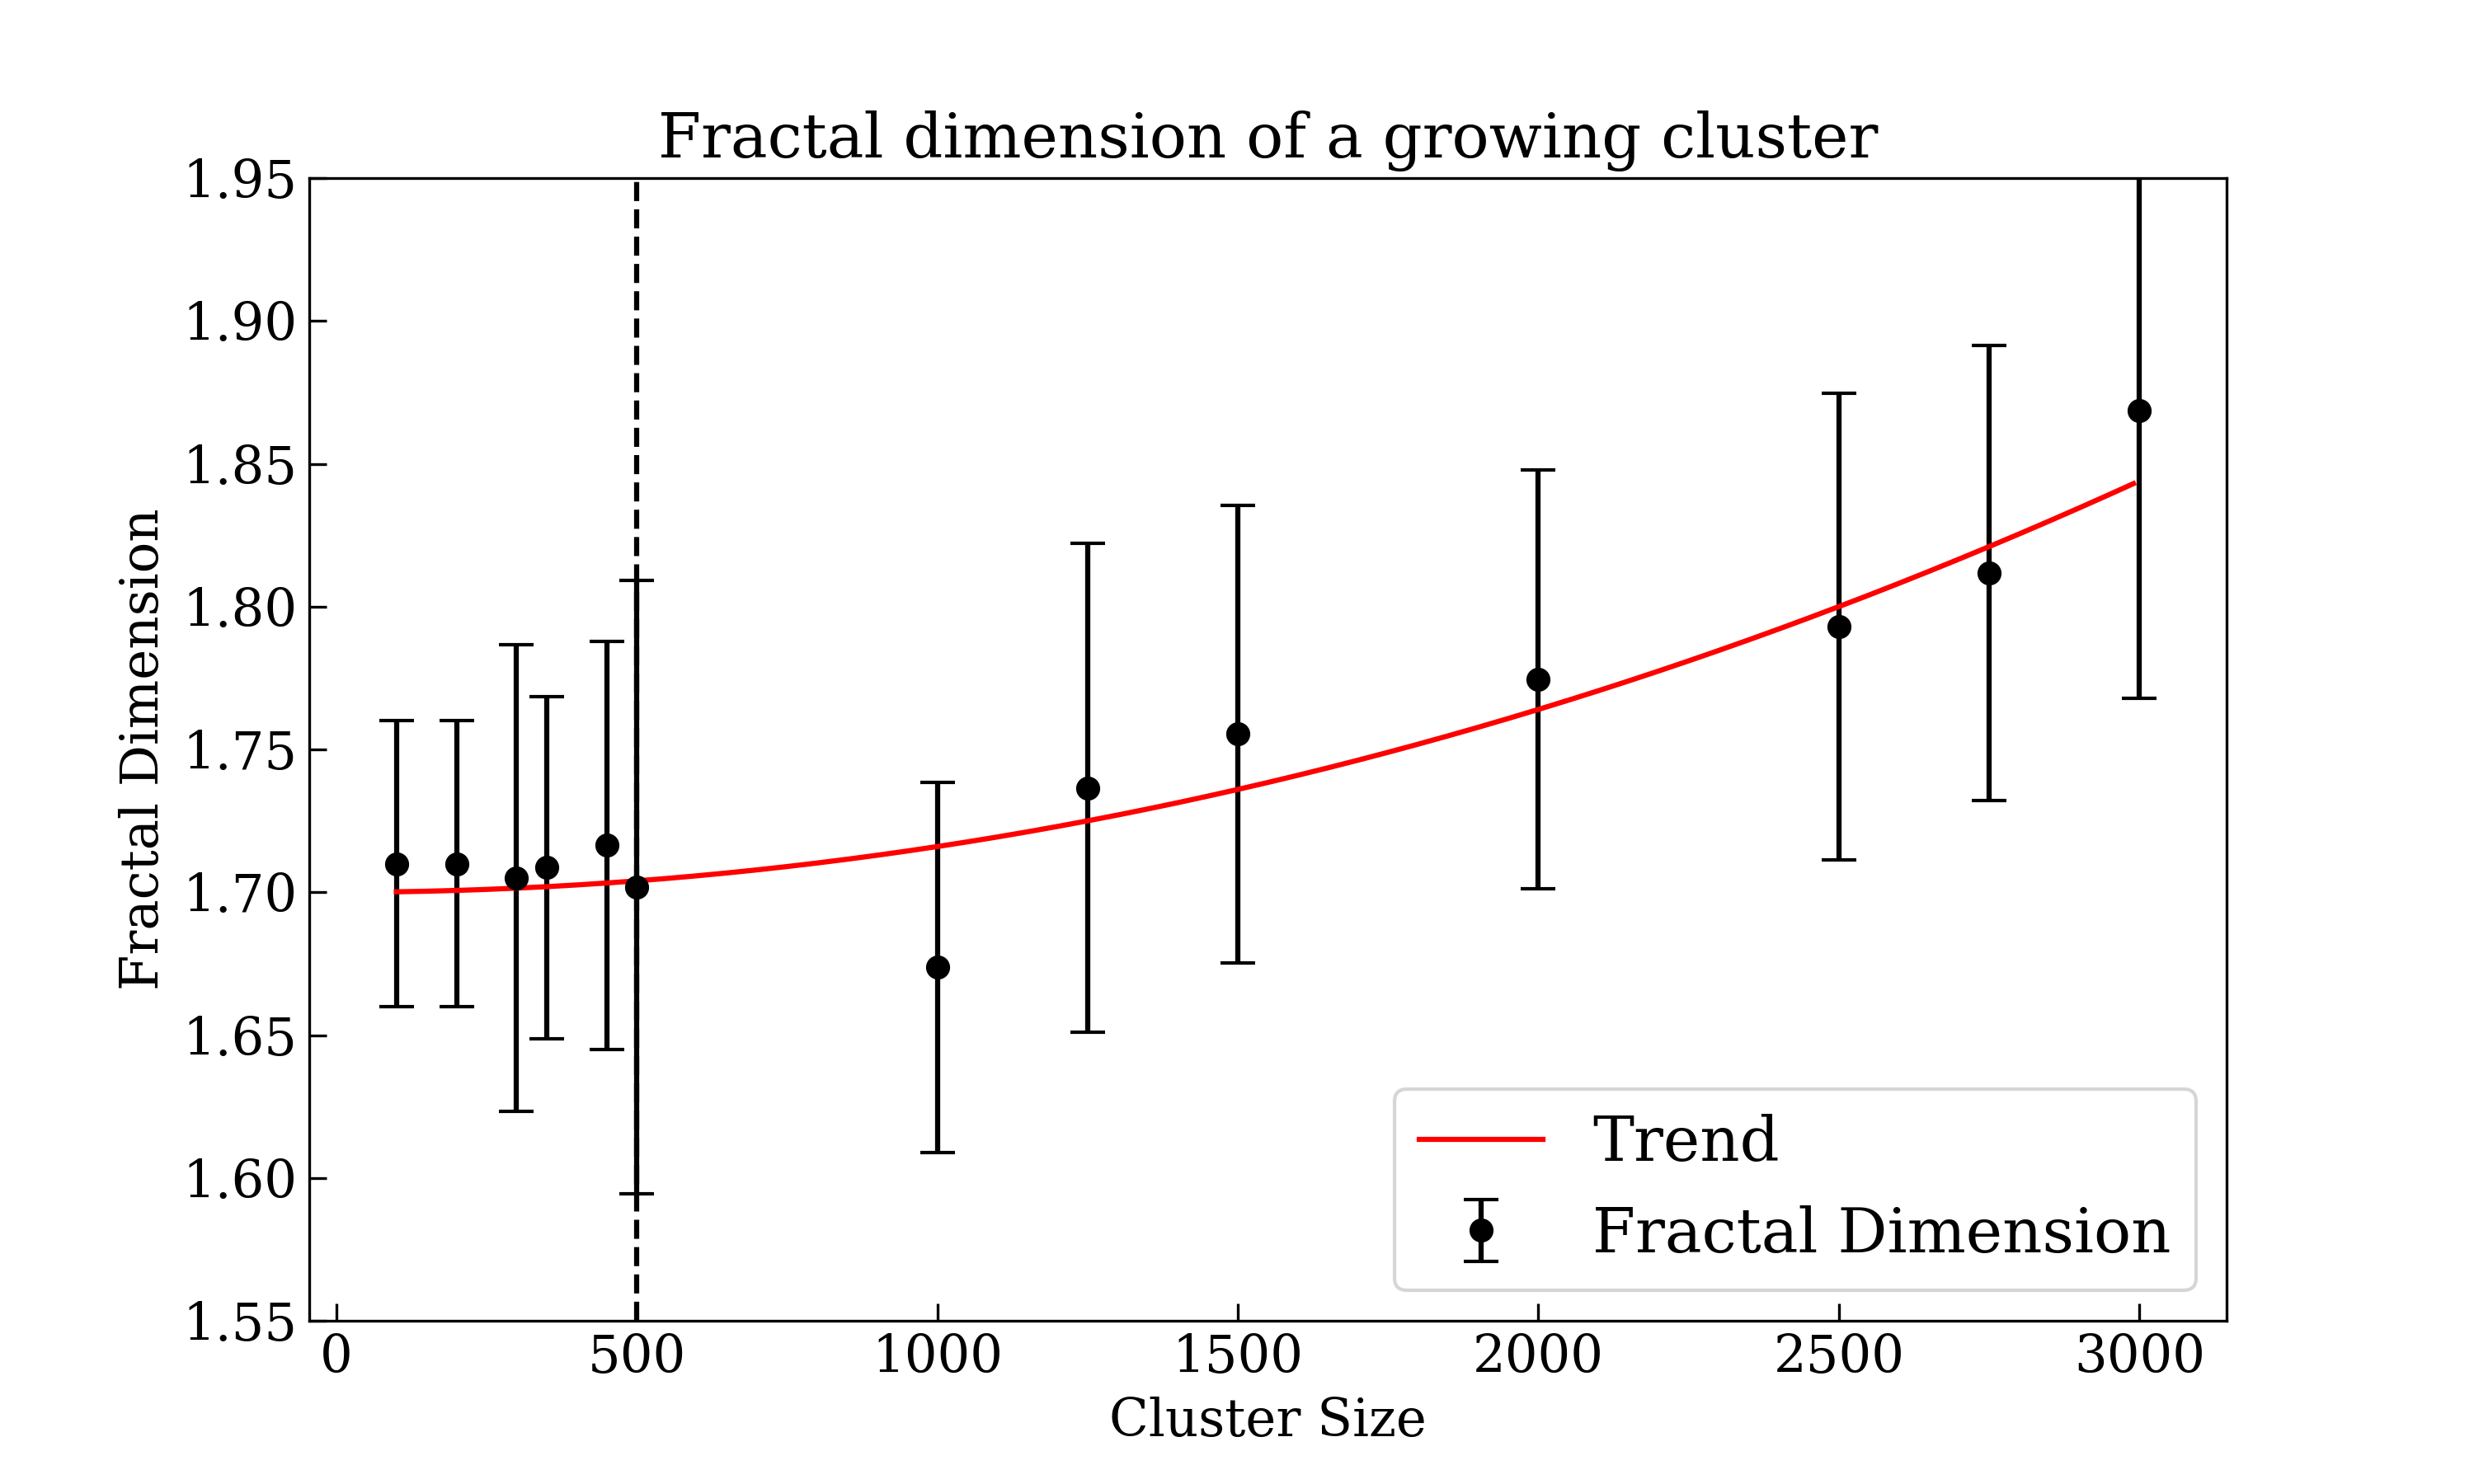
\includegraphics[width=\linewidth]{figures/5.png}
\caption{\label{fig:cluster_growth}A cluster grown at a density of 2\%. At 500 particles the growth will be dominated by particle occupancy. Indeed once the particle reaches this critical size the fractal dimension begins to increase, tending towards 2.}
\end{figure}
Once again, equation \ref{eq:dla_limit} proves itself to be an accurate representation of the system. At a density of 0.02 a cluster of 500 almost particles should remain in diffusion limit. Once the cluster exceeds this critical size its growth will be dominated by the occupancy of nearby states. As expected, figure \ref{fig:cluster_growth} demonstrates this size dependence. Until 500 particles, within measurement uncertainty, the  fractal dimension remains at the literature value of 1.71, beyond this limit the fractal dimension begins to diverge from the diffusion value. In practice, figure \ref{fig:cluster_growth} demonstrates that clusters can be grown to almost twice this size before the fractal dimension changes significantly.

Of note is the size of error bars in figure \ref{fig:cluster_growth}, before 500 particles there is relatively few data points in the linear fit used by the box counting algorithm (as boxes must remain much larger than data points) giving rise to large uncertainties in the measurement uncertainties despite the values not significantly deviating from 1.71. Beyond this critical cluster size error bars are relatively large due to the spectrum of fractal dimensions in the cluster - at the centre there are 500 particles with $d=1.71$ but further out the fractal dimension is higher.
\section{\label{sec:conclusion}Conclusion}
It has been shown in independent simulations that the DLA process proposed by Witten and Sander\cite{WittenDLA} produces a fractal with a dimension consistent with the literature value of 1.71\cite{FractalsBook}. Further modelling changing the probability of a walker joining the cluster causes the fractal dimension of the DLA cluster to tend towards 2 - a results intuitively understood and also visible in visualisations of the simulation. Yet more investigation into the density of walkers, rather than singularly generated particles, gave an equation which can be used to determine the density of walkers for which the process will remain diffusion limited. Beyond the limit found in this equation, the dimension, again, tends towards two. A results caused by the outwards growth of the cluster being dominated by occupied neighbour states rather than diffusion onto the cluster.
%\begin{acknowledgments}
%We wish to acknowledge the support of the author community in using
%\dots.
%\end{acknowledgments}
\newpage

\appendix
\newpage
\section{References \& Footnotes}
\bibliography{references}% Produces the bibliography via BibTeX.
\newpage
\section{\label{ap:witten_dla}DLA Simulation by Witten and Sander}
The following image from Meakin's 1995 paper shows the addition, kill and maximal radius circles of the DLA simulation used by Witten and Sander.
\begin{figure}[h]
\centering
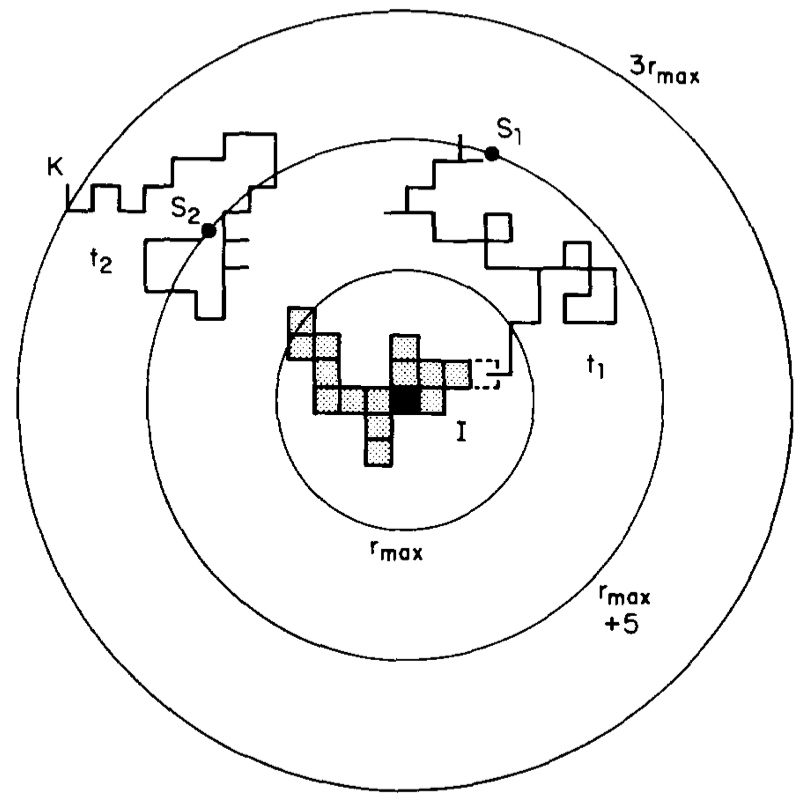
\includegraphics[width=0.8\linewidth]{figures/WittenDLA.png}
\caption{\label{fig:witten_dla_system}Schematic of simulation used by Witten and Sander. Particles are created at $r_{max}+5$ and killed at $3 r_{max}$. Particle $s_1$ is shown joining the cluster and $s_2$ being killed. Image from Meakin 1995\cite{MeakinDLA2}.}
\end{figure}

\subsection{\label{ap:box_counting}Box Counting}

\end{document}
%
% ****** End of file ******
